\section{Spherical geometry \& topology}
\label{sec:geometry}
The most fundamental object with which Driftworld Tectonics works is a mesh of a sphere in the 3D Euclidean space. For simplicity, we assume the sphere is a unit sphere centered on the origin unless stated otherwise. Because of the spherical nature of the project, several (arguably) uncommon mathematical concepts are described in this section -- such as vertex sampling, triangulation, transformations or bounding volume hiearchies.
\subsection{Unity coordinate system}
\label{subsec:unitycoords}
Unity uses a left-handed coordinate system with the \textit{x} axis pointing to the right, \textit{y} axis pointing upwards and \textit{z} axis pointing forward (see Figure \ref{fig:unity-coordinate}). This is reflected in the scenes -- nevertheless, the mathematical expressions of vectors themselves are identical to a standard right-handed coordinate system, i. e. the following holds for the basis:
$$\mathbf{e}_x \times \mathbf{e}_y = \mathbf{e}_z$$
All implementations must be aware of the fact that the cross product expressions do not distinguish between right-handed and left-handed. It is simply a matter of axes display, where visually 'switching' axes \textit{y} and \textit{z} alternates between left-handedness and right-handedness. In the left-handed coordinate system, right-hand rule of cross product shows the inverse final direction of the cross product.
\begin{figure}[ht]
\centering
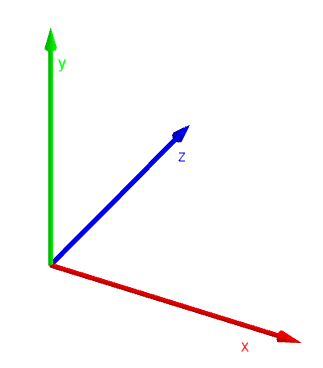
\includegraphics[height=7cm]{unity-axes.png}
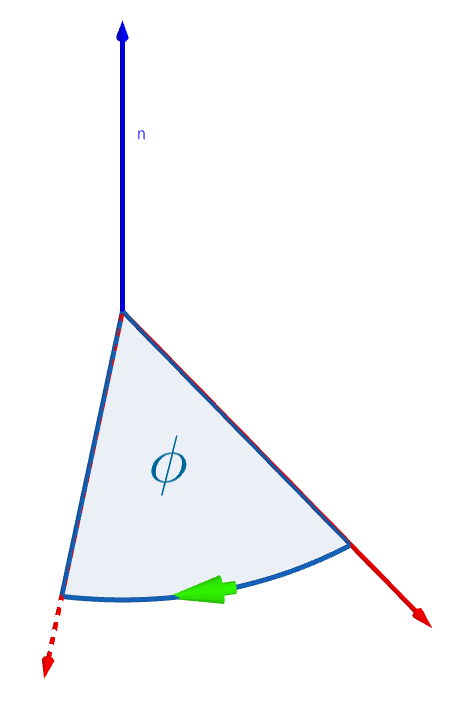
\includegraphics[height=7cm]{unity-rotation.png}
\caption{Unity coordinate system}
\label{fig:unity-coordinate}
\end{figure}

There are several ways to rotate points, vectors or whole transformations. For clarity, let us assume a 3-dimensional vector $\mathbf{u}$ that is to be rotated. We define a rotation unit vector $\mathbf{n}$ and an angle $\phi$ by which we rotate $\mathbf{u}$ so that $\mathbf{u}$ rotates by $\phi$ within a plane to which $\mathbf{n}$ is normal. We also assume that the rotation plane passes through the origin. Then from the perspective of a sundial (with $\mathbf{n}$ being the gnomon) $\mathbf{u}$ rotates \textit{clockwise} for positive $\phi$ (Figure \ref{fig:unity-coordinate}). This holds for all relative rotations.

\subsection{Sectional planes and great circles}
Sphere can have any number of sectional planes, i. e. planes that have some non-empty intersection with the sphere. A subset of planes passing the center of the sphere will be called \textit{sectional central planes} (Figure \ref{fig:sectional-plane}). Any sectional central plane $\rho$ is characterized by some non-zero normal vector $\textbf{n}_\rho$ and for any point on the plane represented by their position vector $\mathbf{x}$ it holds that
$$\mathbf{n}_\rho\cdot\mathbf{x}=0$$
This is synonymous to the fact that any vector lying within a plane passing the origin is perpendicular to the normal vector of the plane. The dot product on the left side of the equality is also important because given a specific normal vector we can decide on which side is any vector $\mathbf{x}$ \textit{outside} the plane -- simply take the sign of the dot product, vector on the side of the normal vector will result in a positive dot product value with $\mathbf{n}_\rho$, negative otherwise.

An important object on the surface of a sphere is a great circle. It is any circle that shares its center and radius with the sphere (Figure \ref{fig:great-circle}). It is also the intersection of a plane passing the center of the sphere with its surface.
\begin{figure}[ht]
\centering
\begin{subfigure}{7cm}
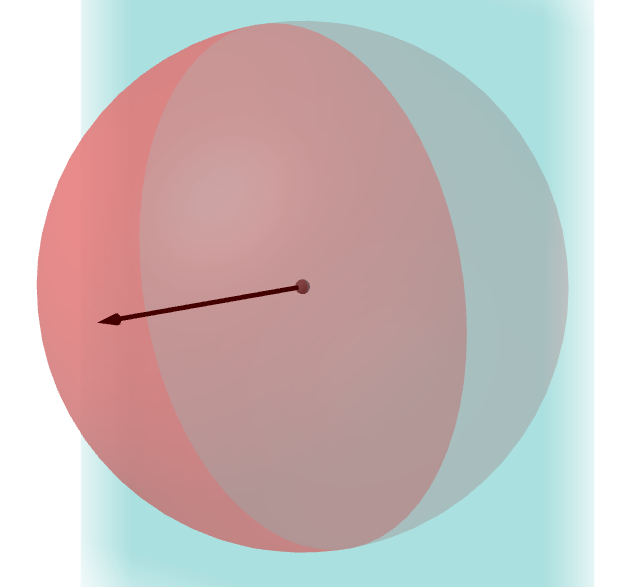
\includegraphics[height=6cm]{sectional-plane.png}
\caption{central plane}
\label{fig:sectional-plane}
\end{subfigure}
\begin{subfigure}{7cm}
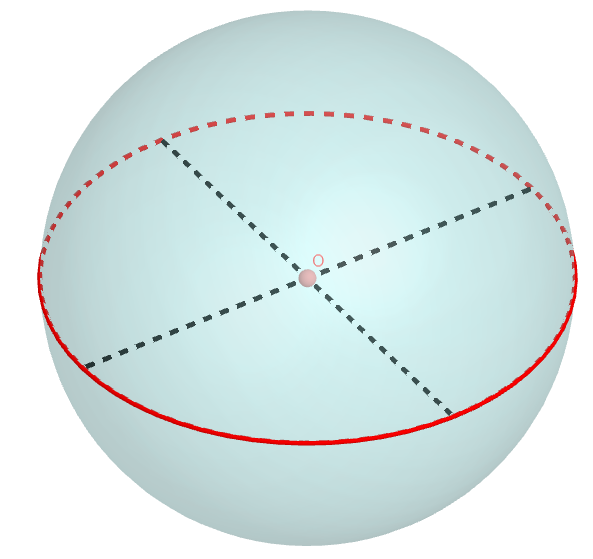
\includegraphics[height=6cm]{great-circle.png}
\caption{great circle}
\label{fig:great-circle}
\end{subfigure}
\caption{Sphere section by plane}
\label{fig:sectional-objects}
\end{figure}

\subsection{Spherical triangles}
Any three points on the surface of a sphere that do not lie on a single great circle form a~\textit{spherical triangle} (Figure \ref{fig:spherical-triangle}). This is the fundamental concept behind many of the computations in the project.

\begin{figure}[ht]
\centering
\begin{subfigure}{7cm}
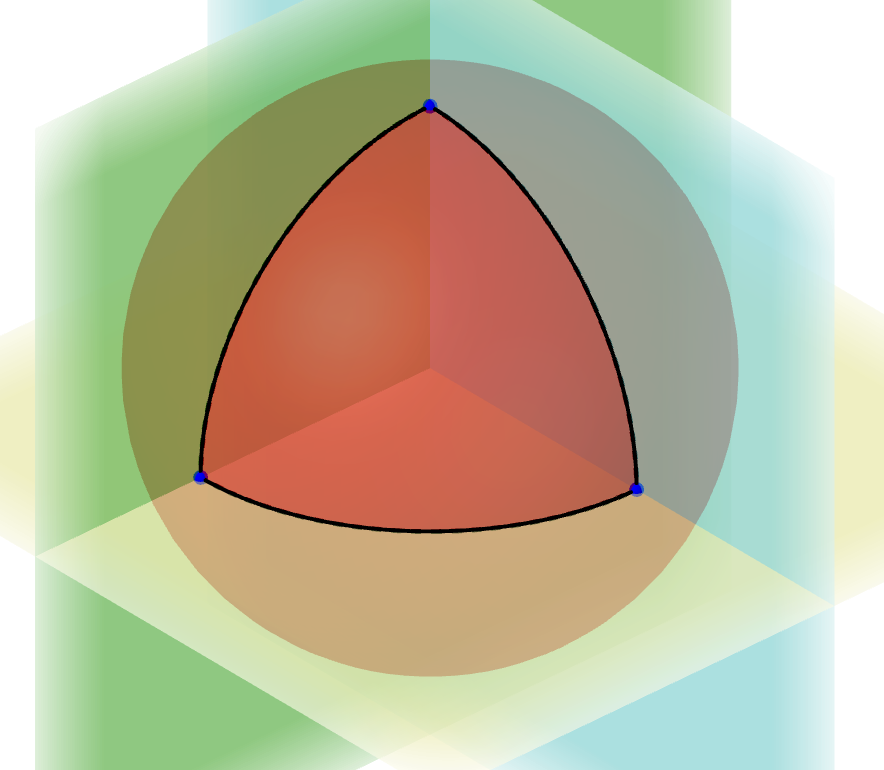
\includegraphics[height=6cm]{triangle.png}
\caption{planes intersections}
\label{fig:spherical-triangle-visual}
\end{subfigure}
\begin{subfigure}{7cm}
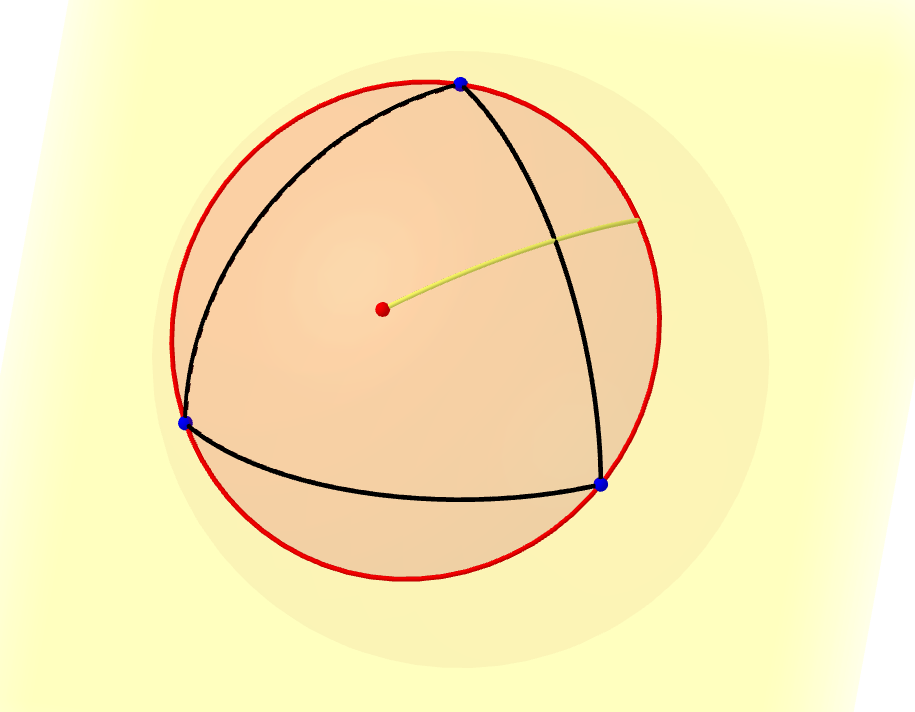
\includegraphics[height=6cm]{triangle-circumcircle.png}
\caption{circumcircle and sectional plane}
\label{fig:triangle-circumcircle}
\end{subfigure}
\caption{Spherical triangle}
\label{fig:spherical-triangle}
\end{figure}

Strictly speaking, there are two triangles defined by such three points. The complement of any spherical triangle with respect to the sphere surface is also a spherical triangle, albeit one of the two is unintuitive. To clarify, we try to formally construct a spherical triangle definition.

Geometrically speaking, a spherical triangle is a region bounded by three arcs of great circles \cite{palmer}. We denote the surface of a unit sphere $\mathcal{S} =  \{\mathbf{x} \in \mathbb{R}^3: ||\mathbf{x}||=1\}$. Given three linearly independent point vectors $\mathbf{a},\mathbf{b},\mathbf{c}\in \mathcal{S}$ we calculate three normal vectors:
$$\mathbf{n}_{\rho}=\mathbf{a}\times\mathbf{b},$$
$$\mathbf{n}_{\sigma}=\mathbf{b}\times\mathbf{c},$$
$$\mathbf{n}_{\tau}=\mathbf{c}\times\mathbf{a}.$$
These vectors define planes $\rho, \sigma, \tau$ so that
$$\rho=\{\mathbf{x}\in\mathbb{R}^3:\mathbf{n}_{\rho}\cdot\mathbf{x}=0\}$$
$$\sigma=\{\mathbf{x}\in\mathbb{R}^3:\mathbf{n}_{\sigma}\cdot\mathbf{x}=0\}$$
$$\tau=\{\mathbf{x}\in\mathbb{R}^3:\mathbf{n}_{\tau}\cdot\mathbf{x}=0\}$$
intersections $\rho\cap\mathcal{S}, \sigma\cap\mathcal{S}, \tau\cap\mathcal{S}$ are then great circles $p,s,t$ that always pass two of the points $\mathbf{a},\mathbf{b},\mathbf{c}$. Because of this, each one is divided by them into two arcs. There is only one triplet of arcs connected by $\mathbf{a},\mathbf{b}$ or $\mathbf{c}$ that forms a region boundary on $\mathcal{S}$ (Figure \ref{fig:spherical-triangle-visual}). Problem is, there are two such regions. We would like our definition to be unambiguous. Because of the way we computed the normal vectors, there is always a subset of $\mathcal{S}$ so that the dot products of any of its elements with $\mathbf{n}_\rho, \mathbf{n}_\sigma$ and $\mathbf{n}_\tau$ all have the same sign.
\subsection{Vertex sampling}
Because of memory restrictions, sphere surface data is represented as a set of sampled points. We can identify these points as position vectors $\mathbf{u}_i$ from the global origin to sample points, resulting in a~sequence $U=\left(\mathbf{u}_i\right)_{i=0}^{N-1}, \mathbf{u}_i \in \mathbb{R}^3, ||\mathbf{u}_i||=1$. Samples are therefore three-dimensional normalized vectors. Driftworld uses spherical Fibonacci sampling \cite{keinert}. To get the sequence $U$, another sequence $F=\left(\mathbf{f}_i\right)_{i=0}^{N-1}$ is first computed, using the following definition:
$$\mathbf{f}_i=(\phi_i, z_i), \phi_i \in \mathbb{R}, z_i \in \mathbb{R},$$
$$\phi_i = 2\pi\left[\frac{i}{\Phi}\right],$$
$$z_i = 1-\frac{2i+1}{N}.$$
$\left[x\right]$ denotes the fractional part of $x$, $\Phi$ is the golden ratio $\Phi=\frac{\sqrt{5}+1}{2}$. The values of $\mathbf{f}_i$ actually lie on a~spiral on the surface of a cylinder with the radius of 1 and the height of 2 \cite{keinert}. $U$ is finally obtained by mapping $\mathbf{f}_i$ values to a unit sphere:
$$\mathbf{u}_i = (\sin{(\arccos{(z_i)})}\cdot\cos{\phi_i}, z_i, \sin{(\arccos{(z_i)})}\cdot\sin{\phi_i})$$
Note that this mapping reflects Unity's axes orientation and the first and the last samples of $U$ do not fall exactly on the poles.
